% !TeX spellcheck = sk_SK-Slovak
\documentclass[a4paper]{article}
\usepackage[slovak]{babel}
\usepackage[utf8]{inputenc}
\usepackage[T1]{fontenc}
\usepackage{a4wide}
\usepackage{amsmath}
\usepackage{amsfonts}
\usepackage{amssymb}
\usepackage{mathrsfs}
\usepackage[small,bf]{caption}
\usepackage{subcaption}
\usepackage{xcolor}
\usepackage{graphicx}
\usepackage{enumerate}
\usepackage{hyperref}
\usepackage{fancyvrb}
\usepackage{listings}
%\usepackage{lstautogobble}
\usepackage{stmaryrd}

\lstset{basicstyle=\ttfamily,
	mathescape=true,
	escapeinside=||%,
	%autogobble
}


\fvset{tabsize=4}


\pagestyle{empty}
\setlength{\parindent}{0pt}

\newenvironment{modenumerate}
{\enumerate\setupmodenumerate}
{\endenumerate}

\newif\ifmoditem
\newcommand{\setupmodenumerate}{%
	\global\moditemfalse
	\let\origmakelabel\makelabel
	\def\moditem##1{\global\moditemtrue\def\mesymbol{##1}\item}%
	\def\makelabel##1{%
		\origmakelabel{##1\ifmoditem\rlap{\mesymbol}\fi\enspace}%
		\global\moditemfalse}%
}

\makeatletter
\def\@seccntformat#1{%
	\expandafter\ifx\csname c@#1\endcsname\c@section\else
	\csname the#1\endcsname\quad
	\fi}
\makeatother

\begin{document} 
	
\pagenumbering{arabic}
\pagestyle{plain}

\begin{center}
	\sc\large
	Algoritmické riešenia ťažkých problémov\\
	Domáca úloha 2
\end{center}

Autor: Marián Kravec

\section{Úloha 2 - Vertex cover, independent set, and clique}

\subsection*{a)}

Ako prvé si ukážme, že vieme v polynomiálnom čase vytvoriť komplementárny graf. Keďže komplementárny graf má rovnakú množinu vrcholov ako pôvodný graf stačí nám pre každú dvojicu vrcholov skontrolovať či medzi nimi existuje hrana ak v novom grafe vytvoriť opak, aj keby sme kontrolovali existenciu hrany triviálne prejdením všetkých hrán zložitosť by bola O($m n^2$) ($m$ ako počet hrán a $n^2$ ako počet dvojíc vrcholov) čiže to vieme zhora ohraničiť na O($n^4$) (keďže kompletný graf má nanajvýš $\frac{n(n-1)}{2}$ hrán čiže približne O($n^2$)). 
\\

Čiže vidíme, že polynomiálna transformácia grafu je možná, takže vieme v polynomiálnom čase nájsť najväčšiu nezávislú množinu komplementu grafu, teraz potrebujeme dokázať, že najväčšia nezávislá množina na komplemente grafu je najväčší clique v pôvodnom grafe. Keďže vieme, že každá nezávislá množina v komplemente je clique v pôvodnom grafe (tvrdenie zo zadania úlohy) stačí nám dokázať, že tento clique je najväčší. Toto dokážeme sporom.
\\

Uvažujme, že náš algoritmus nám vrátil nezávislú množinu v komplemente o veľkosti $k$, z toho vyplýva, že v pôvodnom grafe je to clique o veľkosti $k$, keďže tvrdíme, že tento clique nie je najväčší tak tvrdíme, že v grafe existuje clique o veľkosti $l$ pričom $l > k$. Keďže každý clique je kompletný graf tak clique veľkosti $l$ obsahuje aj clique všetkých veľkostí od 1 po $l$, preto bez ujmy na všeobecnosti môžeme tvrdiť, že v grafe existuje clique veľkosti $k+1$. Týchto $k+1$ vrcholov tvorí kompletný podgraf (keďže clique musí byť plne prepojený) preto v komplementárnom grafe medzi tými vrcholmi nemôže existovať žiadna hrana (ak by existovala nemohla by existovať v pôvodnom grafe a podgraf by nemohol byť kompletný). Keďže v komplementárnom grafe neexistuje žiadne hrana medzi týmito vrcholmi tvoria nezávislú množiny, keďže ich je $k+1$ tak aj veľkosť tejto množiny je $k+1$ čo je však SPOR s tým, že najväčšia nezávislá množina v komplemente je $k$ keďže $k+1>k$. 

Z toho vyplýva, že najväčšia nezávislá množina komplementu je najväčší clique v pôvodnom grafe. $\oblong$
\\

Takže vieme, že ak algoritmus hľadajúci najväčšiu nezávislú množinu spustíme, na komplemente grafu dostaneme najväčší clique v pôvodnom grafe. $\oblong$
\\

Teraz prejdime na tvrdenie Prof. Knowitall o tom, že tvrdenie platí aj pre $\frac{1}{i}$-aproximačný algoritmus. Toto tvrdenie je pravdivé, keďže výsledná množina vrcholov je totožná pre nezávislú množinu v komplemente a clique v pôvodnom. Inými slovami keby sme mali $\frac{1}{i}$-aproximačný algoritmus na riešenie nezávislej množiny a najväčšia nezávislá množina komplementu má veľkosť $k$ tak náš aproximačný algoritmus nájde množinu ktorej veľkosť je aspoň $APXALG\_IS(G)\geq\frac{k}{i}$. Inými slovami (keďže komplement grafu vieme vypočítať v polynomiálnom čase) nájde clique ktorého veľkosť je $APXALG\_CL(G)\geq\frac{k}{i}$ a keďže vieme, že najväčší clique je rovnako veľký ako najväčšia nezávislá množina komplementu čiže tiež $k$ vieme o aproximačnom algoritme $APXALG\_CL(G)$ tvrdiť, že polynomiálny (s polynomialnou redukciu algoritmu $APXALG\_IS(G)$) a je i-aproximačný. $\oblong$
\newpage

\subsection*{b)}

Túto úlohu budeme riešiť podobne ako predchádzajúcu. Znovu vieme, že ak množina $U$ je nezávislá množina tak množina $V-U$ je vrcholové pokrytie (tvrdenie zo zadania). Takže zase potrebujeme dokázať iba to, že ak $U$ ($|U|=k$) je najväčšia nezávislá množina tak $V-U$ ($|V-U|=n-k$) je najmenšie vrcholové pokrytie, a znova to dokážeme sporom.
\\

Takže tvrdíme, ak $U$ je najväčšia nezávislá množina veľkosti $|U|=k$ tak existuje vrcholové pokrytie $W$ ktorého veľkosť je $|W|<n-k$, čiže menšia ako počet vrcholov ktoré nepatria do $U$.Znovu bez ujmy na všeobecnosti môžeme uvažovať, že keďže existuje vrcholové pokrytie s veľkosťou $|W|<n-k$ tak musí existovať vrcholové pokrytie s veľkosťou $|W|=n-k-1=n-(k+1)$ (keďže veľkosť môže byť iba prirodzené číslo a menšiemu vrcholovému pokrytiu vieme pridávať body bez toho aby sme porušili pravidlo vrcholového pokrytia). Takže existuje $k+1$ vrcholov ktoré do tohto vrcholové pokrytia nepatria. Keďže aj bez týchto vrcholov sú pokryté všetky hrany musí pre každý z týchto vrcholov platiť, že všetci ich susedia patria do množiny $W$ (čiže vrcholové pokrytia), v opačnom prípade by hrana spájajúca tieto vrcholy nebola pokrytá. Z toho vyplýva, že máme $k+1$ vrcholov ktoré nemôžu mať žiadnu spoločnú hranu (lebo by tá hrana nebola pokrytá) čiže tvoria nezávislú množinu. To je však SPOR s tvrdením, že množina $U$ ktorej veľkosť je $|U|=k$ je najväčšou nezávislou množinou grafu keďže $k+1>k$.

Z toho vyplýva, že vrcholy ktoré nepatria do najväčšej nezávislej množiny tvoria najmenšie vrcholové pokrytie v grafe. $\oblong$
\\

Takže vieme, že ak algoritmus hľadajúci najväčšiu nezávislú množinu spustíme, na grafe a výslednú množinu odčítame od množiny všetkých vrcholov dostaneme najmenšie vrcholové pokrytie v grafe. $\oblong$
\\

Teraz sa pozrieme na tvrdenie Prof. Knowitall o tom, že tvrdenie platí aj pre $\frac{1}{i}$-aproximačný algoritmus. V tomto prípade, toto tvrdenie nie je pravdivé. Ukážeme si to na príklade. Majme takýto graf s dvanástimi vrcholmi, a majme $\frac{1}{2}$-aproximačný, ktorý vyberie vrcholy následne:


\centerline{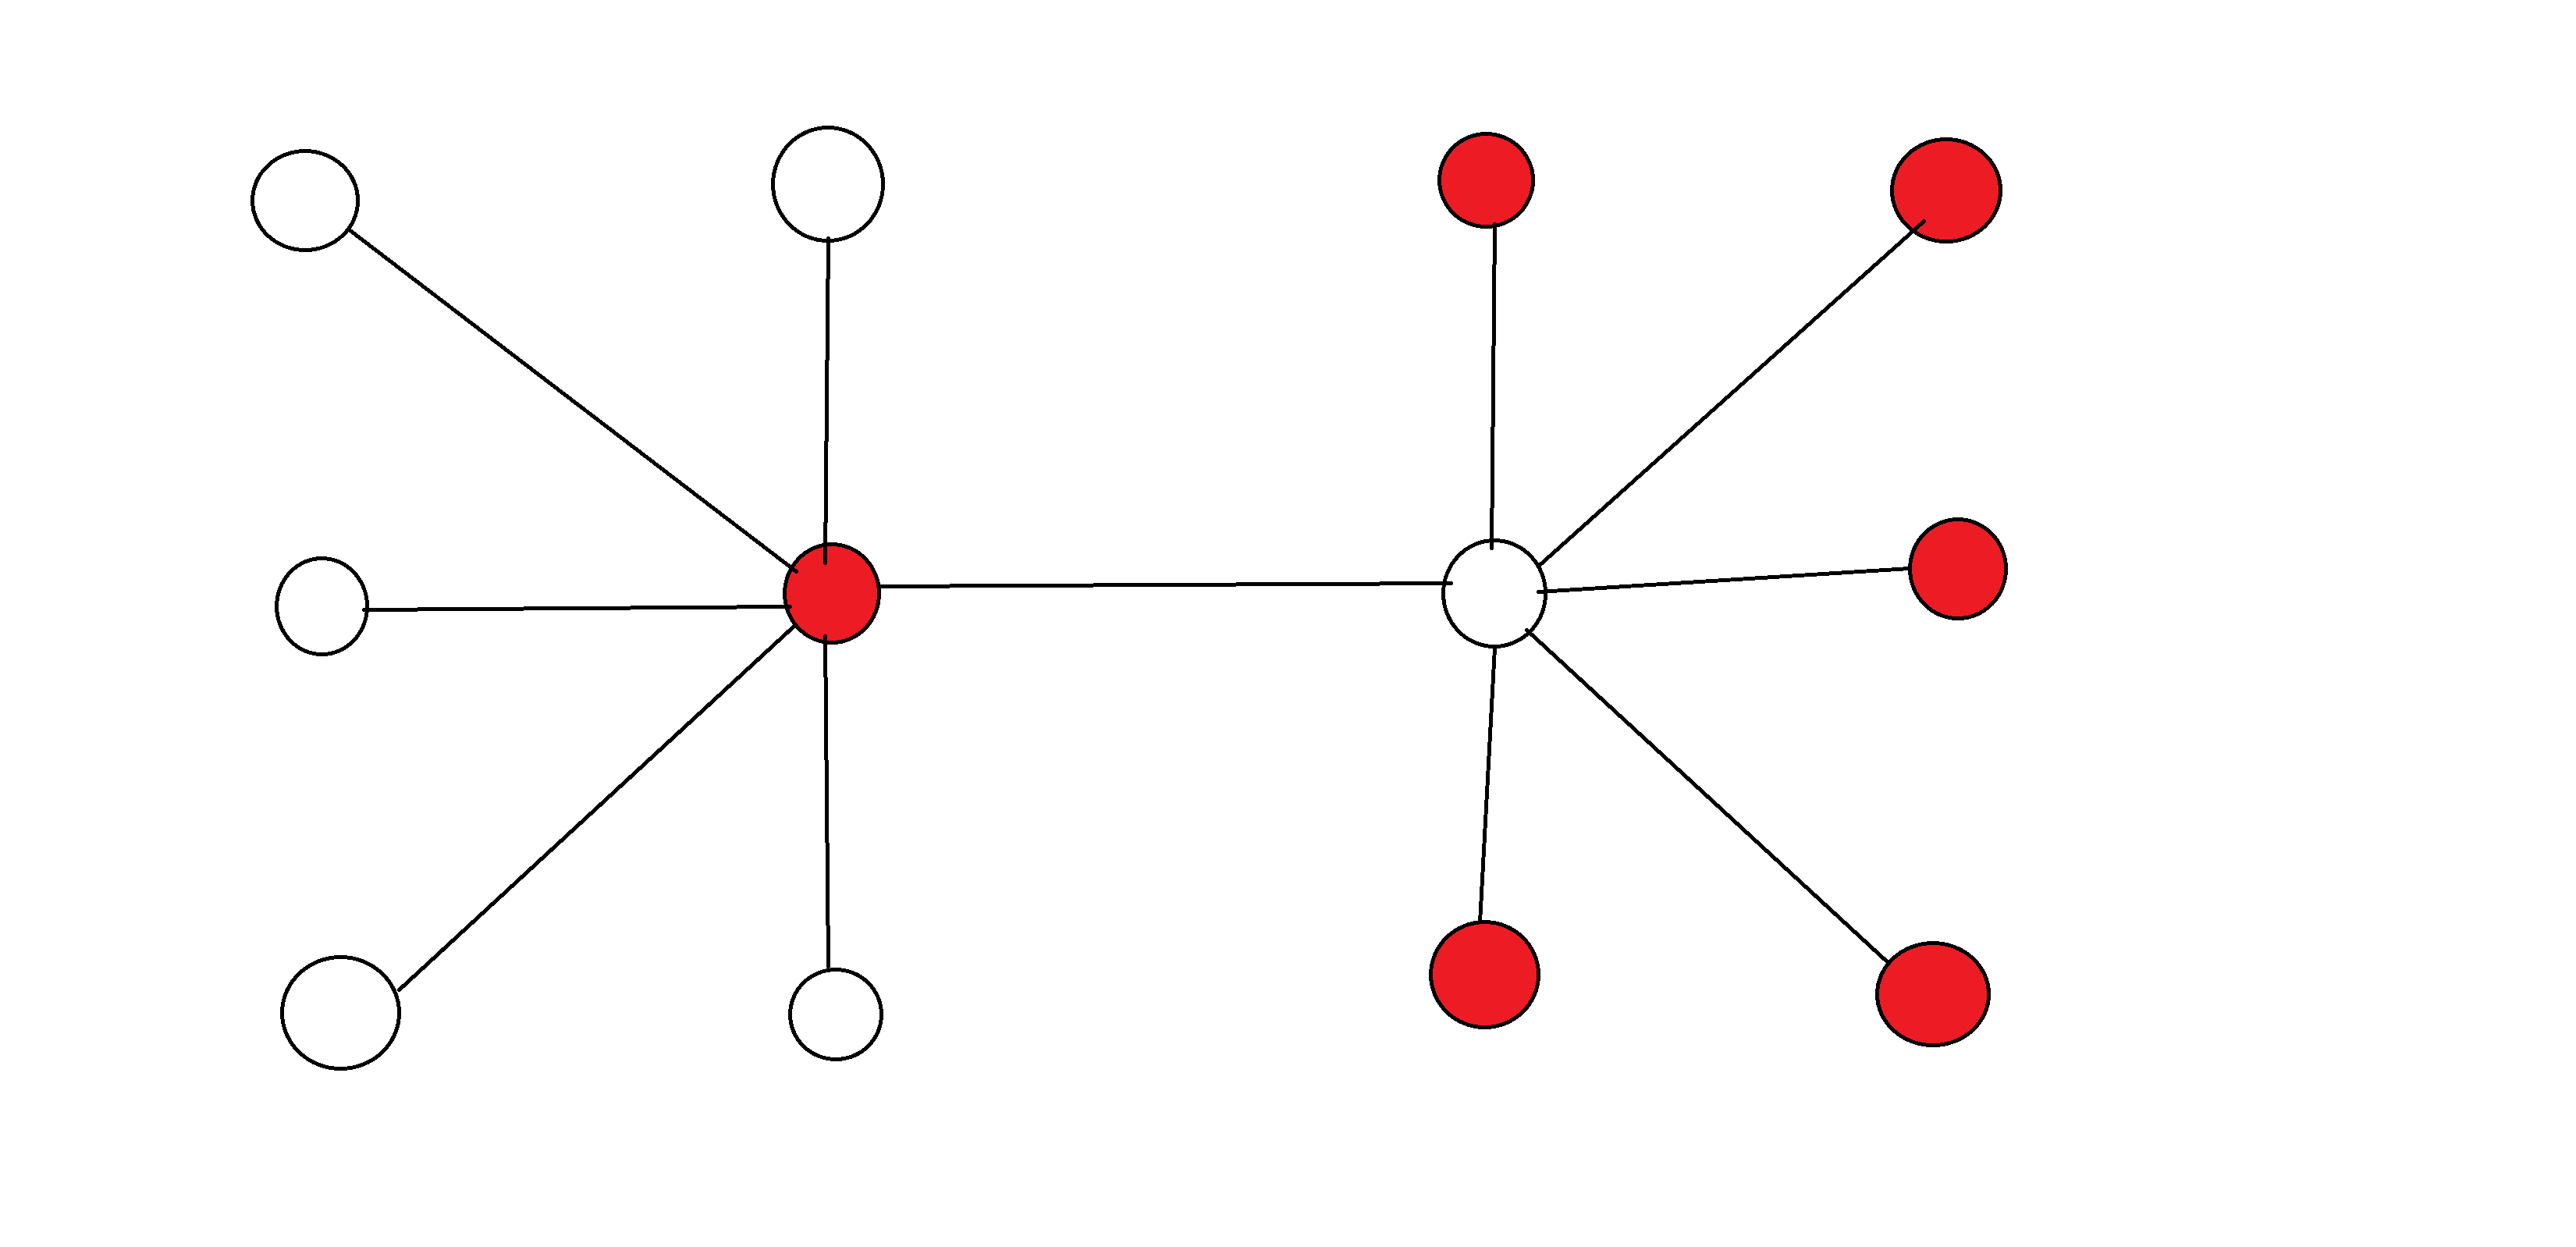
\includegraphics[width=0.8\textwidth]{12}}

Na tomto jednoduchom grafe vidíme, optimálna nezávislá množina má veľkosť 10 (všetky vrcholy okrem dvoch stredových) náš aproximačný algoritmus však vybral 6 vrcholov (označené na červeno) čím spĺňa $\frac{1}{2}$-aproximačný faktor keďže $\frac{6}{10} > \frac{1}{2}$. Najmenšie vrcholové pokrytie je v tomto prípade 2 (iba stredové vrcholy) ale náš algoritmus vybral 6 (všetky neoznačené na červeno keďže tie netvoria nezávislú množinu a naša polynomialna redukcia algoritmu hovorí, že výsledok pre vrcholové pokrytie sú vrcholy nepatriace do nezávislej množiny), z tohto by vyplýva, že pri najlepšom by náš algoritmus bol $\frac{6}{2}$ čiže 3-aproximačný. Teraz zachovajme štruktúra grafu tak, že existujú 2 stredové vrcholy a z nich vychádzajú hrany k vrcholom stupňa 1 pričom z oboch vychádza rovnaký počet hrán a zachovajme aj výsledok algoritmu pre nezávislú množinu tak, že zoberie jeden stredový vrchol a všetky okolité k druhému stredovému a jediné čo zmeníme je počet vrcholov stupňa jedna ku každému stredovému vrcholu na arbitrárnu hodnotu $n$. Tým dostaneme graf ktorý má $2n+2$ vrcholov a takýto výsledok algoritmu pre nezávislú množinu:

\centerline{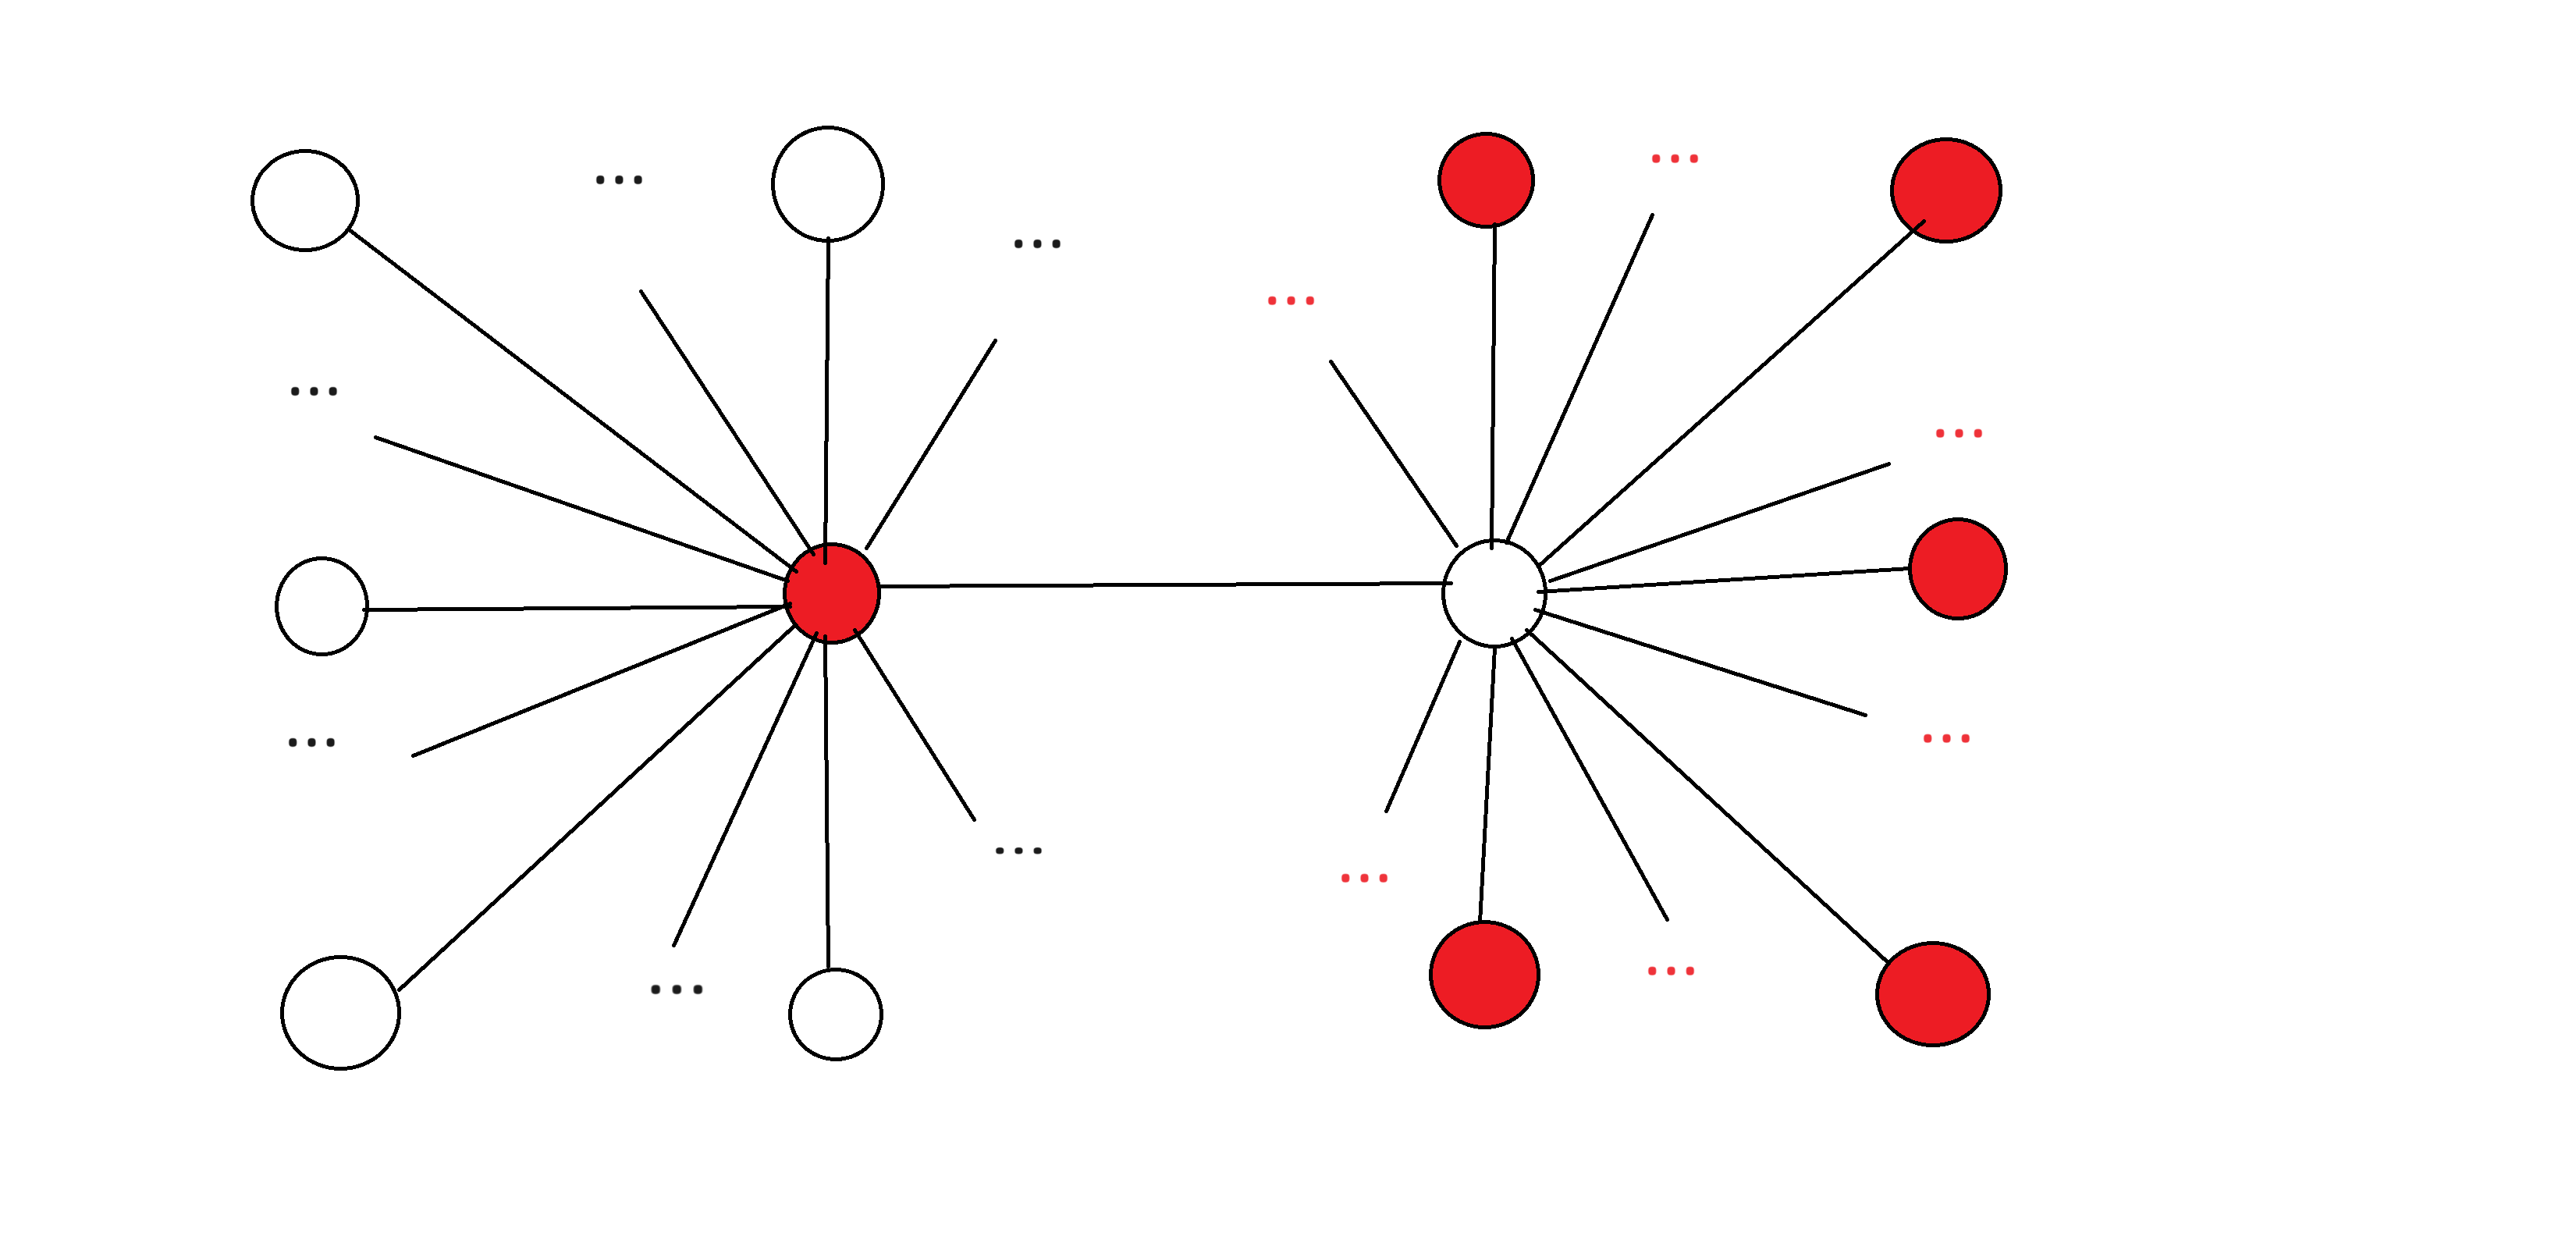
\includegraphics[width=0.8\textwidth]{2n2}}

V tomto grafe stále platí, že najväčšia nezávislá množina je tvorená všetkými vrcholmi okrem dvoch stredových čiže jej veľkosť je $2m$, náš algoritmus vybral okolité vrcholy jedného stredového vrcholu (je ich $m$) a druhý stredový čiže dohromady $m+1$, čím stále spĺňa $\frac{1}{2}$-aproximačný faktor keďže $\frac{m+1}{2m} > \frac{m}{2m} = \frac{1}{2}$ avšak najmenšie vrcholové pokrytie je stále 2 (iba stredové vrcholy) ale algoritmus vráti $m+1$ vrcholov (znovu je neoznačený jeden stredový a okolie druhého stredového). Z toho by vyplývalo, že náš algoritmus má pre najmenšie vrcholové pokrytie prinajlepšom $\frac{m+1}{2}$-aproximačný faktor, avšak keďže $m$ môže byť arbitrárne veľké tento faktor nemôže byť konštantný, takže aj napriek tomu, že máme $\frac{1}{2}$-aproximačný algoritmus pre nezávislú množinu tento algoritmus nemá konštantný aproximačný faktor pre problém vrcholového pokrytie.
\\

Pevne verím, že toto je dostatočný kontrapríklad.

\end{document}